\section{Methodology}
\label{sec:method}
As illustrated in Figure~\ref{fig:Pipeline},  DEFEND's core consists of four agent components, SimulationAgent and RevisionAgent areoptional and are designed to further expand the usability of the framework. Pipeline is presented in Appendix~\ref{appendix:pipeline} and detailed prompts of each module are provided in Appendix~\ref{appendix:prompt}.
\begin{figure}
    \centering
    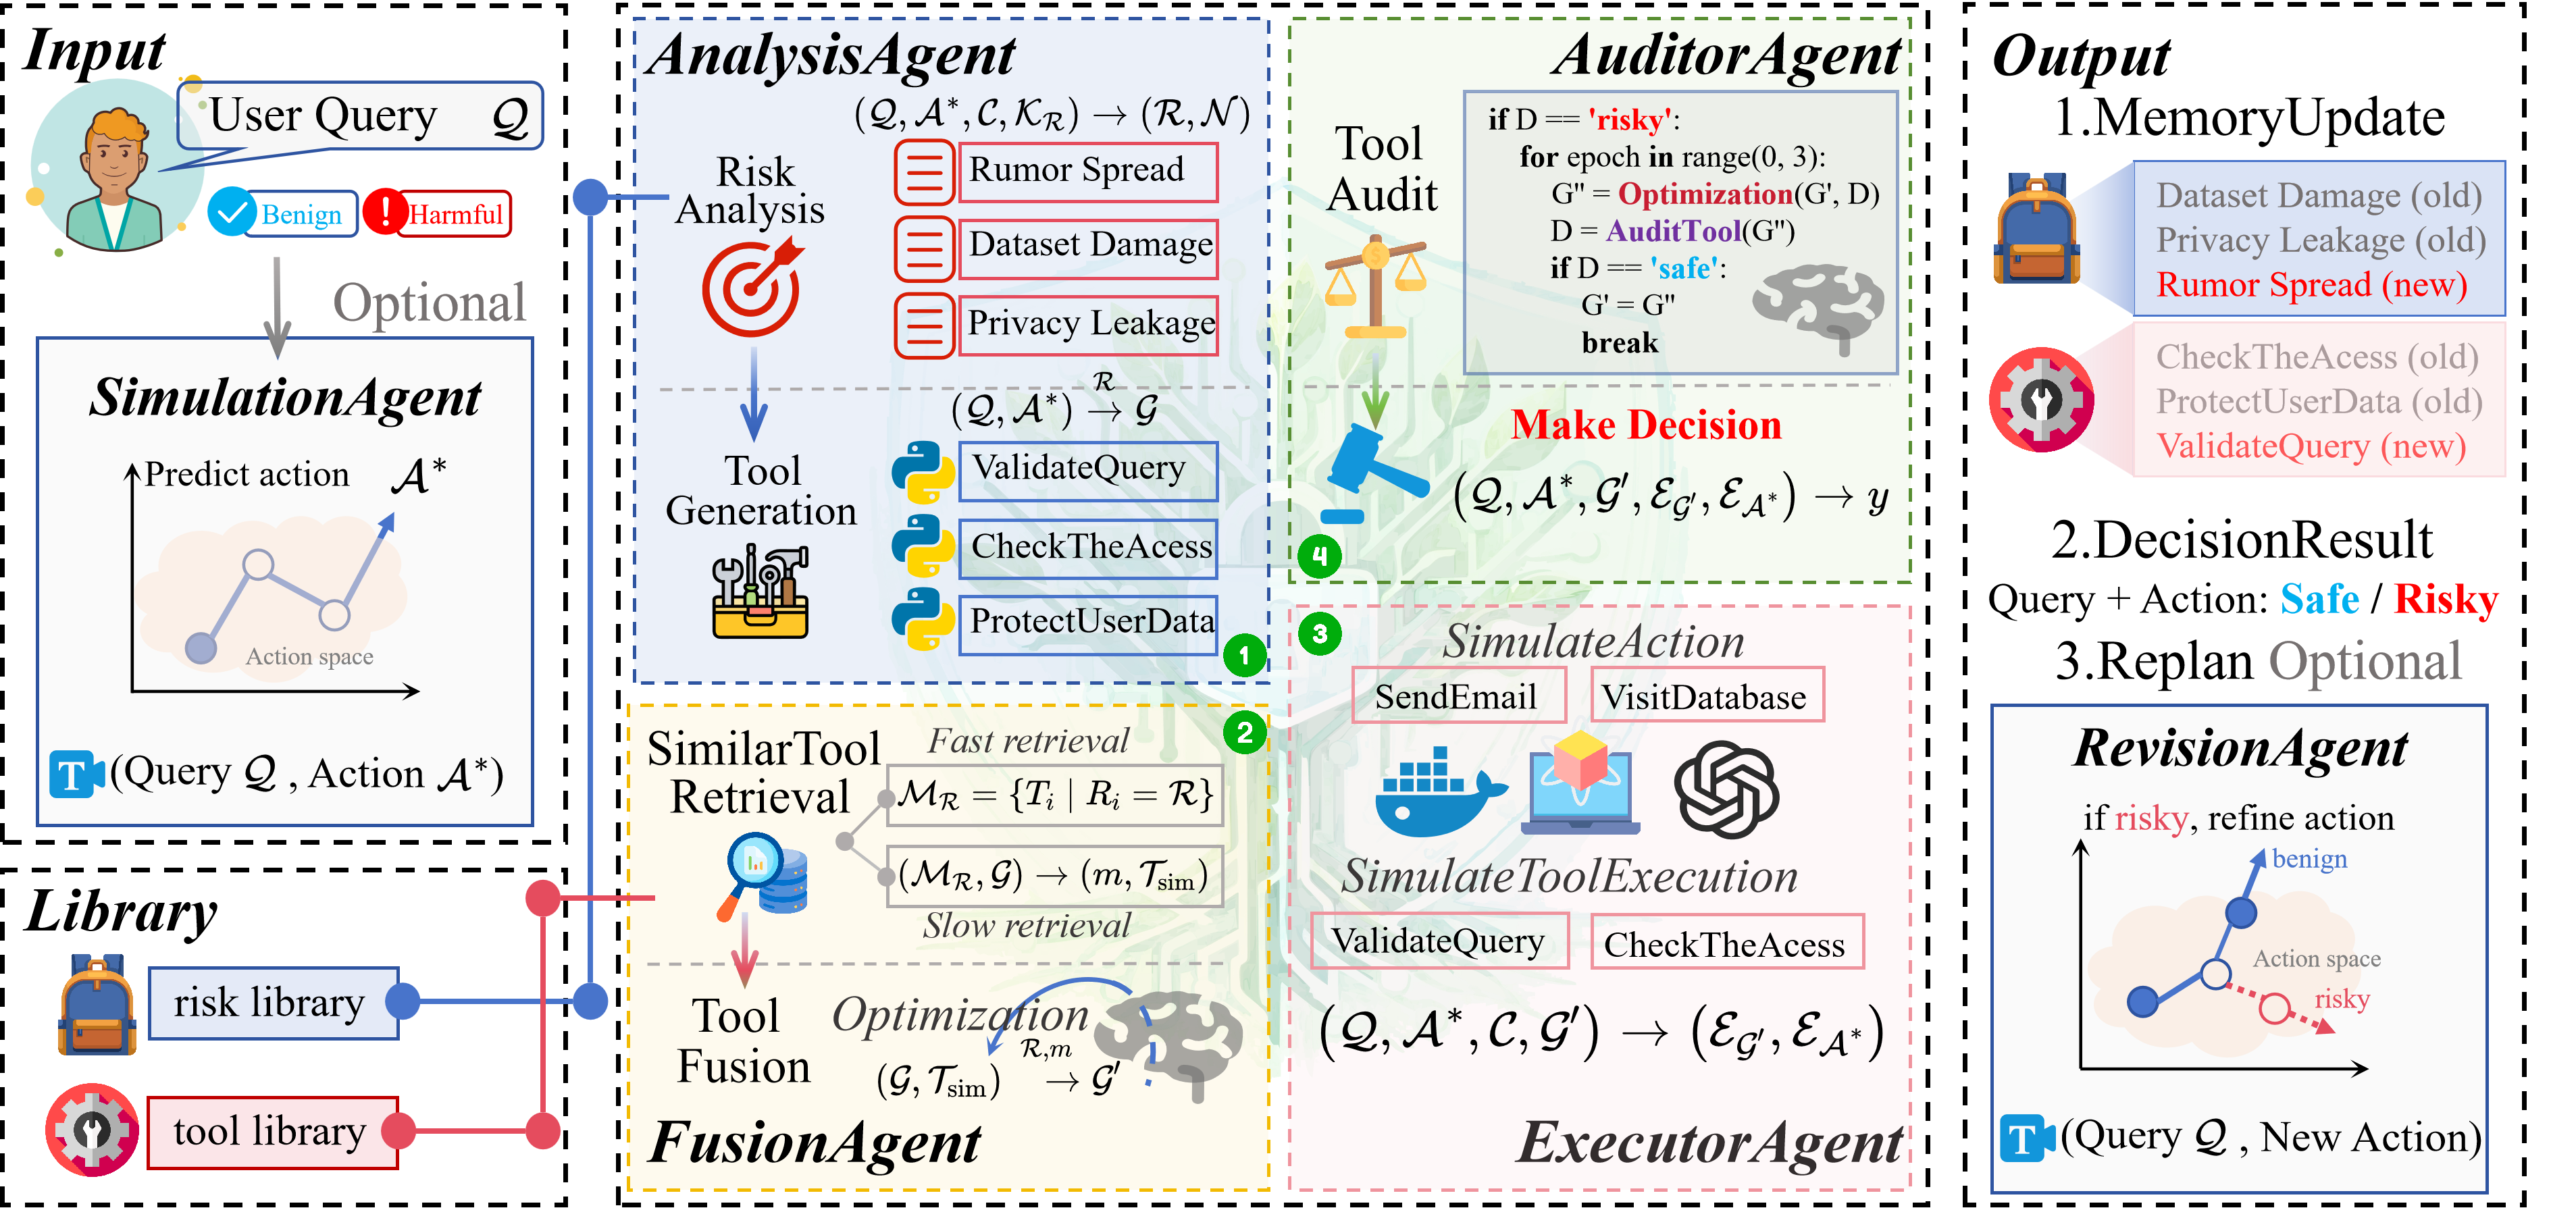
\includegraphics[width=\linewidth]{code/pipeline.png}
    \caption{DEFEND's framework.}
    \label{fig:Pipeline}
\end{figure}
\subsection{SimulationAgent}
SimulationAgent is an \emph{optional} front-end module designed to simulate real agent operations. In standard DEFEND process, inputs are user queries $\mathcal{Q}$ and the protected agent's intended action $\mathcal{A^*}$. When DEFEND only receives $\mathcal{R}$ and lacks clearly agent action $\mathcal{A^*}$, the optional SimulationAgent module is activated to bridge the gap between the user's intent and the specific agent action.

Given natural language user queries $\mathcal{Q}$, SimulationAgent utilizes its internal LLM and agent's action space $\mathcal{A}$, predict ordered actions $\mathcal{A^*}$ that real agent will take to complete the queries under model parameters $\theta$:
\begin{equation}
    \mathcal{A^*}=\arg\max_{A\in\mathcal{A}} P \left( A\mid \mathcal{Q};\theta \right).
\end{equation}
$\mathcal{R}$ is combined with $\mathcal{A^*}$ to form a structured tuple ($\mathcal{R}$, $\mathcal{A^*}$ ), which serves as the input for AnalysisAgent.


\subsection{AnalysisAgent}
AnalysisAgent receives $\mathcal{Q}$ and $\mathcal{A^*}$, with the environment $\mathcal{C}$, first performs risk analysis. We define $\mathcal{K_R}$ as lifelong risk knowledge library, $\mathcal{R}$ as the risk category (existing or new), and $\mathcal{N} \in \{0,1\}$ as whether security tools are needed. The risk analysis process is:
\begin{equation}
    \text{Risk Analysis:} \quad \left(\mathcal{Q},\mathcal{A^*},\mathcal{C},\mathcal{K_R}\right) \xrightarrow{} \left(\mathcal{R},\mathcal{N} \right).
\end{equation}
If security tools are needed for agent protection, AnalysisAgent generates targeted guardrail tools $\mathcal{G}$ based on risk categories $\mathcal{R}$, the process can be represented as:
\begin{equation}
    \text{Tool Generation:}\quad (\mathcal{Q},\mathcal{A^*}) \xrightarrow{\mathcal{R}} \mathcal{G}
\end{equation}


\subsection{FusionAgent}
The core objective of FusionAgent is to maximize the reusability and functional completeness of existing guardrail tools, while avoiding unnecessary tool redundancy. We define lifetime guardrail tool library $\mathcal{K_G} = \left\{\left(T_{i}, R_{i}, \phi_{i}\right)\right\}_{i=1}^{N}$, where $T_i$ is audited python guardrail tool, $R_i$ is the main risk category targeted by the tool, $\phi_i$ is the tool's specific information. FusionAgent retrieves existing tools similar to the new tool and attempt to fuse them to achieve reuse and evolution. 

We design a hierarchical tool retrieval system to accelerate the retrieval process. First, based on $\mathcal{R}$, a candidate subset of existing tools $\mathcal{M_R}$ is quickly filtered out:
\begin{equation}
    \text{Quick Retrieval:}\quad \mathcal{M_R} = \left\{ T_{i} \mid R_{i} = \mathcal{R} \right\}.
\end{equation}
The similar tools should have the same targeted risk category with the new tool, which can be achieved through quick retrieval. For retrieval within the candidate subset, unlike traditional practice leveraging embeddings' similarity, which is sensitive to threshold, we model the retrieval process as an LLM search function, where $m \in \{0,1\}$ indicates whether a reusable match exists, $\mathcal{T_{\text{sim}}}$ is the most similar tool matched when $m = 1$ else empty:
% \begin{equation}
%     \mathcal{J}_{\text{LLM}} : \left(\mathcal{M_R}, \mathcal{G}\right) \rightarrow \left(m, \mathcal{T}_{\text{sim}}\right).
% \end{equation}
\begin{equation}
    \text{Slow Retrieval:}\quad \left(\mathcal{M_R}, \mathcal{G}\right) \rightarrow \left(m, \mathcal{T}_{\text{sim}}\right).
\end{equation}
If $\mathcal{T}_{\text{sim}}$ exists, FusionAgent will reuse and optimize it, integrating the functionality of new tool $\mathcal{G}$ to form new guardrail tool $\mathcal{G}'$, thus achieving efficient tool reuse. Otherwise, $\mathcal{G}$ will be retained as a new guardrail tool. Regardless of reuse, the tools will be validated downstream:
\begin{equation}
    \text{Tool Optimization:} \quad \left( \mathcal{G}, \mathcal{T}_{\text{sim}} \right) \xrightarrow{\mathcal{R}, m} \mathcal{G}'.
\end{equation}


\subsection{ExecutorAgent}
ExecutorAgent acts as a sandbox environment, designed for secure verification and execution in an isolated setting. Its functions include: \ding{172} \emph{Tool execution}: Execute guardrail tool $\mathcal{G}'$ from FusionAgent with user query $\mathcal{Q}$ and agent's intended actions $\mathcal{A}^*$; \ding{173} \emph{Agent's action execution}: Execute agent's intened action based on environment $\mathcal{C}$. The process can be defined below, where $\mathcal{E}_{\mathcal{G}'}$ means tool execution result and $\mathcal{E}_{\mathcal{A}^*}$ stands for agent execution result:
\begin{equation}
    \text{Sandbox Execution:} \quad \left( \mathcal{Q},\mathcal{A}^*,\mathcal{C},\mathcal{G}' \right) \xrightarrow{} \left( \mathcal{E}_{\mathcal{G}'},\mathcal{E}_{\mathcal{A}^*} \right).
\end{equation}
Ruan~\citep{ruan2023identifying} identifies the risks of agents with an LLM-Emulated sandbox, we apply this idea. We also provide a Docker environment for execution in reality.

\subsection{AuditorAgent}
AuditorAgent's core responsibilities include conducting independent and prudent security audits of guardrail tools $\mathcal{G}'$. It combines the tool itself with its execution results to examine through the perspective of vulnerabilities and risks, forming audit result $\mathcal{D} \in \{0,1\}$, 1 means passing auditing. Only tools that pass the audit are allowed to be added to the lifelong tool library $\mathcal{K}_\mathcal{G}$. If tool fails the audit, AuditorAgent will perform secondary optimization based on $\mathcal{D}$ and discard tools that still pose risks after secondary optimization, we define the optimized tool as $\mathcal{G}''$:
\begin{equation}
    \text{Tool Optimization:} \quad \left( \mathcal{G}', \mathcal{D} \right) \xrightarrow{} \mathcal{G}''.
\end{equation}
Thus, we form a strict knowledge update mechanism:
\begin{equation}
    \text{Memory Update: }\quad \mathcal{K}_\mathcal{G} \leftarrow \mathcal{K}_\mathcal{G} \cup \left\{ \mathcal{G}' \mid \mathcal{D}=1 \right\} \cup \left\{ \mathcal{G}'' \mid \mathcal{D}=1 \right\}.
\end{equation}
In addition to tool auditing, AuditorAgent is also responsible for integrating security signals from all modules to make the final decision on whether the query $\mathcal{Q}$ and agent action $\mathcal{A}^*$ is safe or not, defined as label $y$:
\begin{equation}
    \text{Final Decision:} \quad \left( \mathcal{Q},\mathcal{A}^*, \mathcal{G}',\mathcal{E}_{\mathcal{G}'},\mathcal{E}_{\mathcal{A}^*} \right) \xrightarrow{} y.
\end{equation}
By explicitly decoupling tool verification and final judgment, AuditorAgent acts as a ``safety anchor'' in DEFEND. Even if upstream modules introduce potential defects during tool generation or optimization, AuditorAgent can still prevent the adoption of insecure tools based on execution evidence and conservative auditing principles, thereby effectively suppressing agent misevolution caused by the VGT phenomenon, some experimental procedures are presented in Appendix~\ref{appendix:VGT}.

\subsection{RevisionAgent}
RevisionAgent is an \emph{optional} module. RevisionAgent can replan and generate safe actions $\mathcal{A}'$ based on the risks $\mathcal{R}$ of the current query $\mathcal{Q}$ and operation $\mathcal{A}^*$, combined with the action space $\mathcal{A}$. This module extends the DEFEND framework, making it not only limited to a binary judgment of whether something is safe or not, but also able to provide targeted suggestions and mitigation for dangerous operations.
\begin{equation}
    \text{Revision:} \quad \left( \mathcal{Q},\mathcal{{A}^*},\mathcal{R} \right) \xrightarrow{} \mathcal{A'}.
\end{equation}

In conclusion, DEFEND offers the following advantages: (a) Emerging risks identification; (b) Tool generation and reuse; (c) Tool evolution and validation; and (d) Knowledge updating and lifelong learning—all without human intervention.